\section{N-grams language models}\label{sec:n-grams}

An n-gram is a contiguous sequence of items (typically letters or words) that are extracted from an information source (normally text, speech, images or \gls{dna}). By counting the n-grams in a knowledge corpus they can be used to create probabilistic language models for predicting the next item given a context. This is useful when developing speech recognizers and \gls{ocr} systems because the n-gram language model can help disambiguate items in the recognition process. Moreover they can be used for implementing text generators or suggestion / auto-complete systems and can also be applied to improve the efficiency of compression / search algorithms.



\subsection{Rank-frequency graphs}

Rank-frequency graphs are useful to analyze the word / n-gram diversity of a given text corpus. They are usually plotted in logarithmic scale and have the word rank in the X axis and the word frequency in the Y axis. They are also useful to check if a given text corpus follows the Zipf's law \cite{Piantadosi2014}, which states that the frequency of a given word in a text corpus is inversely proportional to its rank in the frequency table (as shown in \cref{eq:zipf-law}).

\begin{equation}\label{eq:zipf-law}
f(r) \propto \frac{1}{r^\alpha}
\end{equation}

Analyzing \crefrange{fig:rank-frequency-unigram}{fig:rank-frequency-pentagram} it can be seen that the dataset unigrams to pentagrams follow roughly the Zipf's law. Moreover, the alpha value introduced in \cref{eq:zipf-law} that best fits the plotted data starts at 0.25 in the first plot section, then increases to 0.5 in the middle plot section and becomes 1.0 in the last plot section. This is a typical behavior found in most languages \cite{NemethZainko2003}.

\begin{figure}[hb]
	\centering
	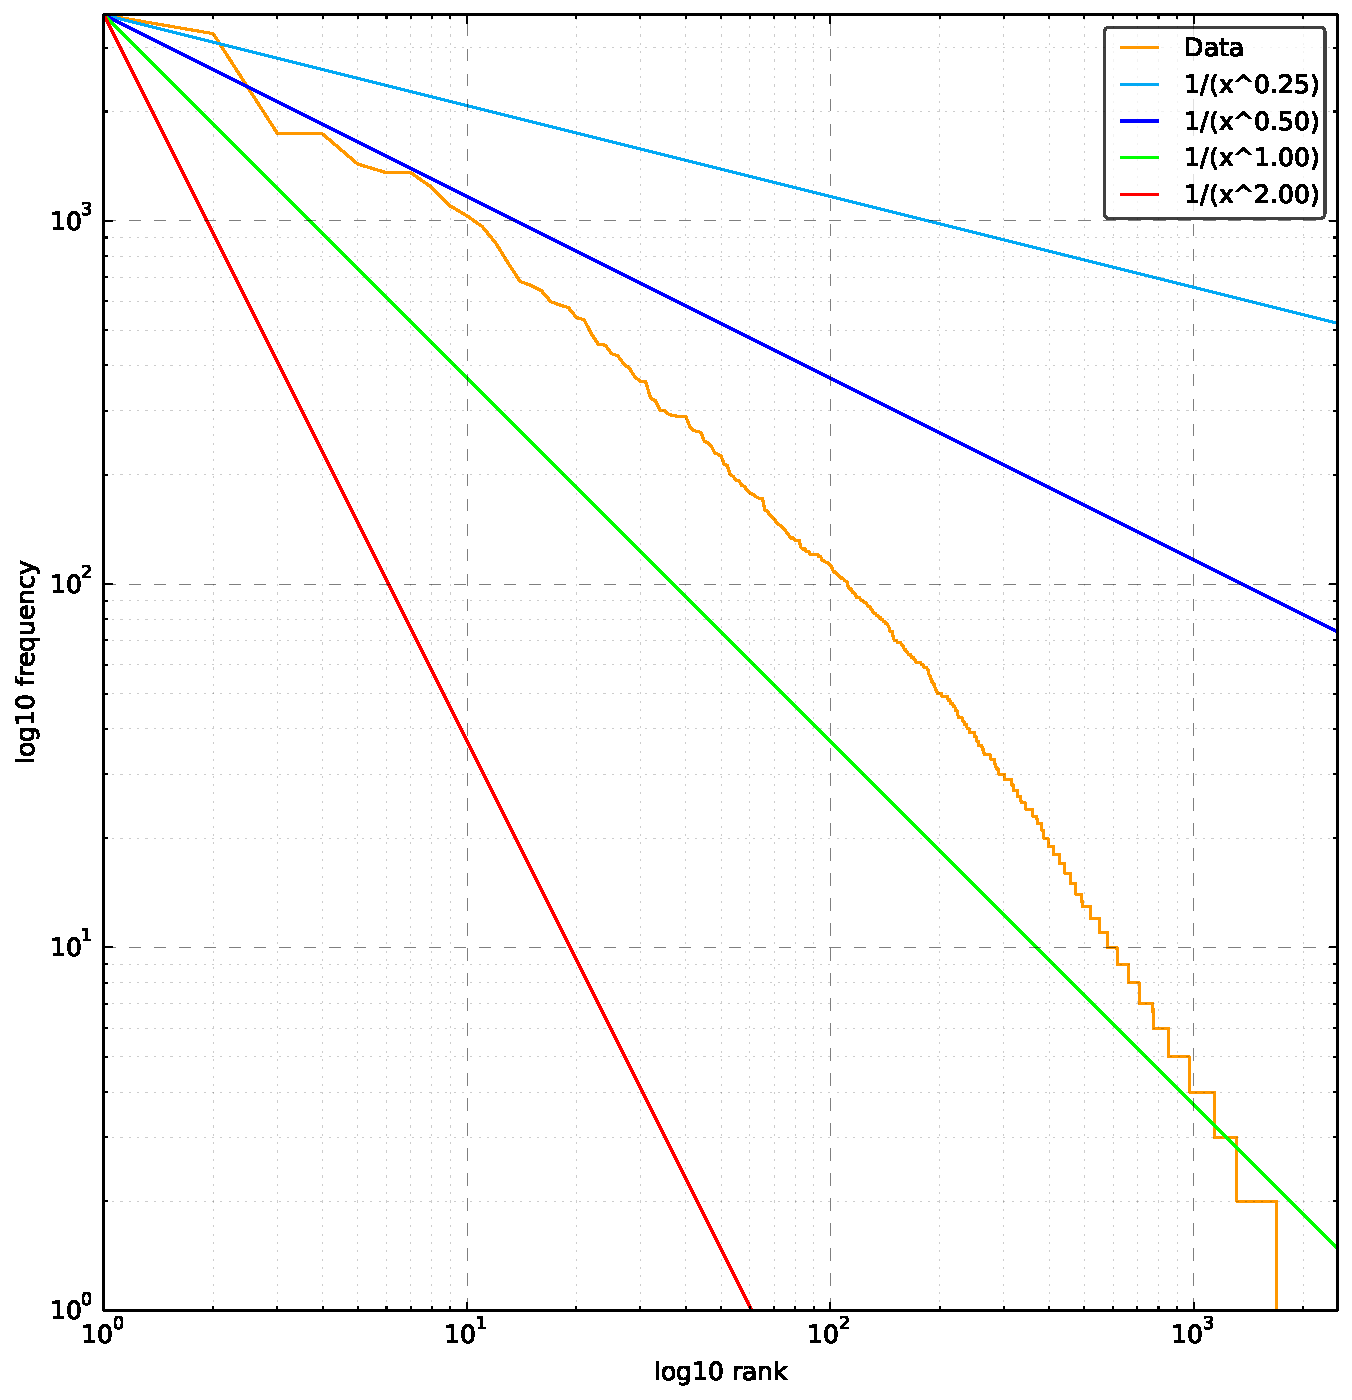
\includegraphics[width=0.9\linewidth]{figures/frequency-graphs/1-gram}
	\caption{Unigram rank-frequency graph of tokenized dataset}
	\label{fig:rank-frequency-unigram}
\end{figure}

\begin{figure}[ht]
	\centering
	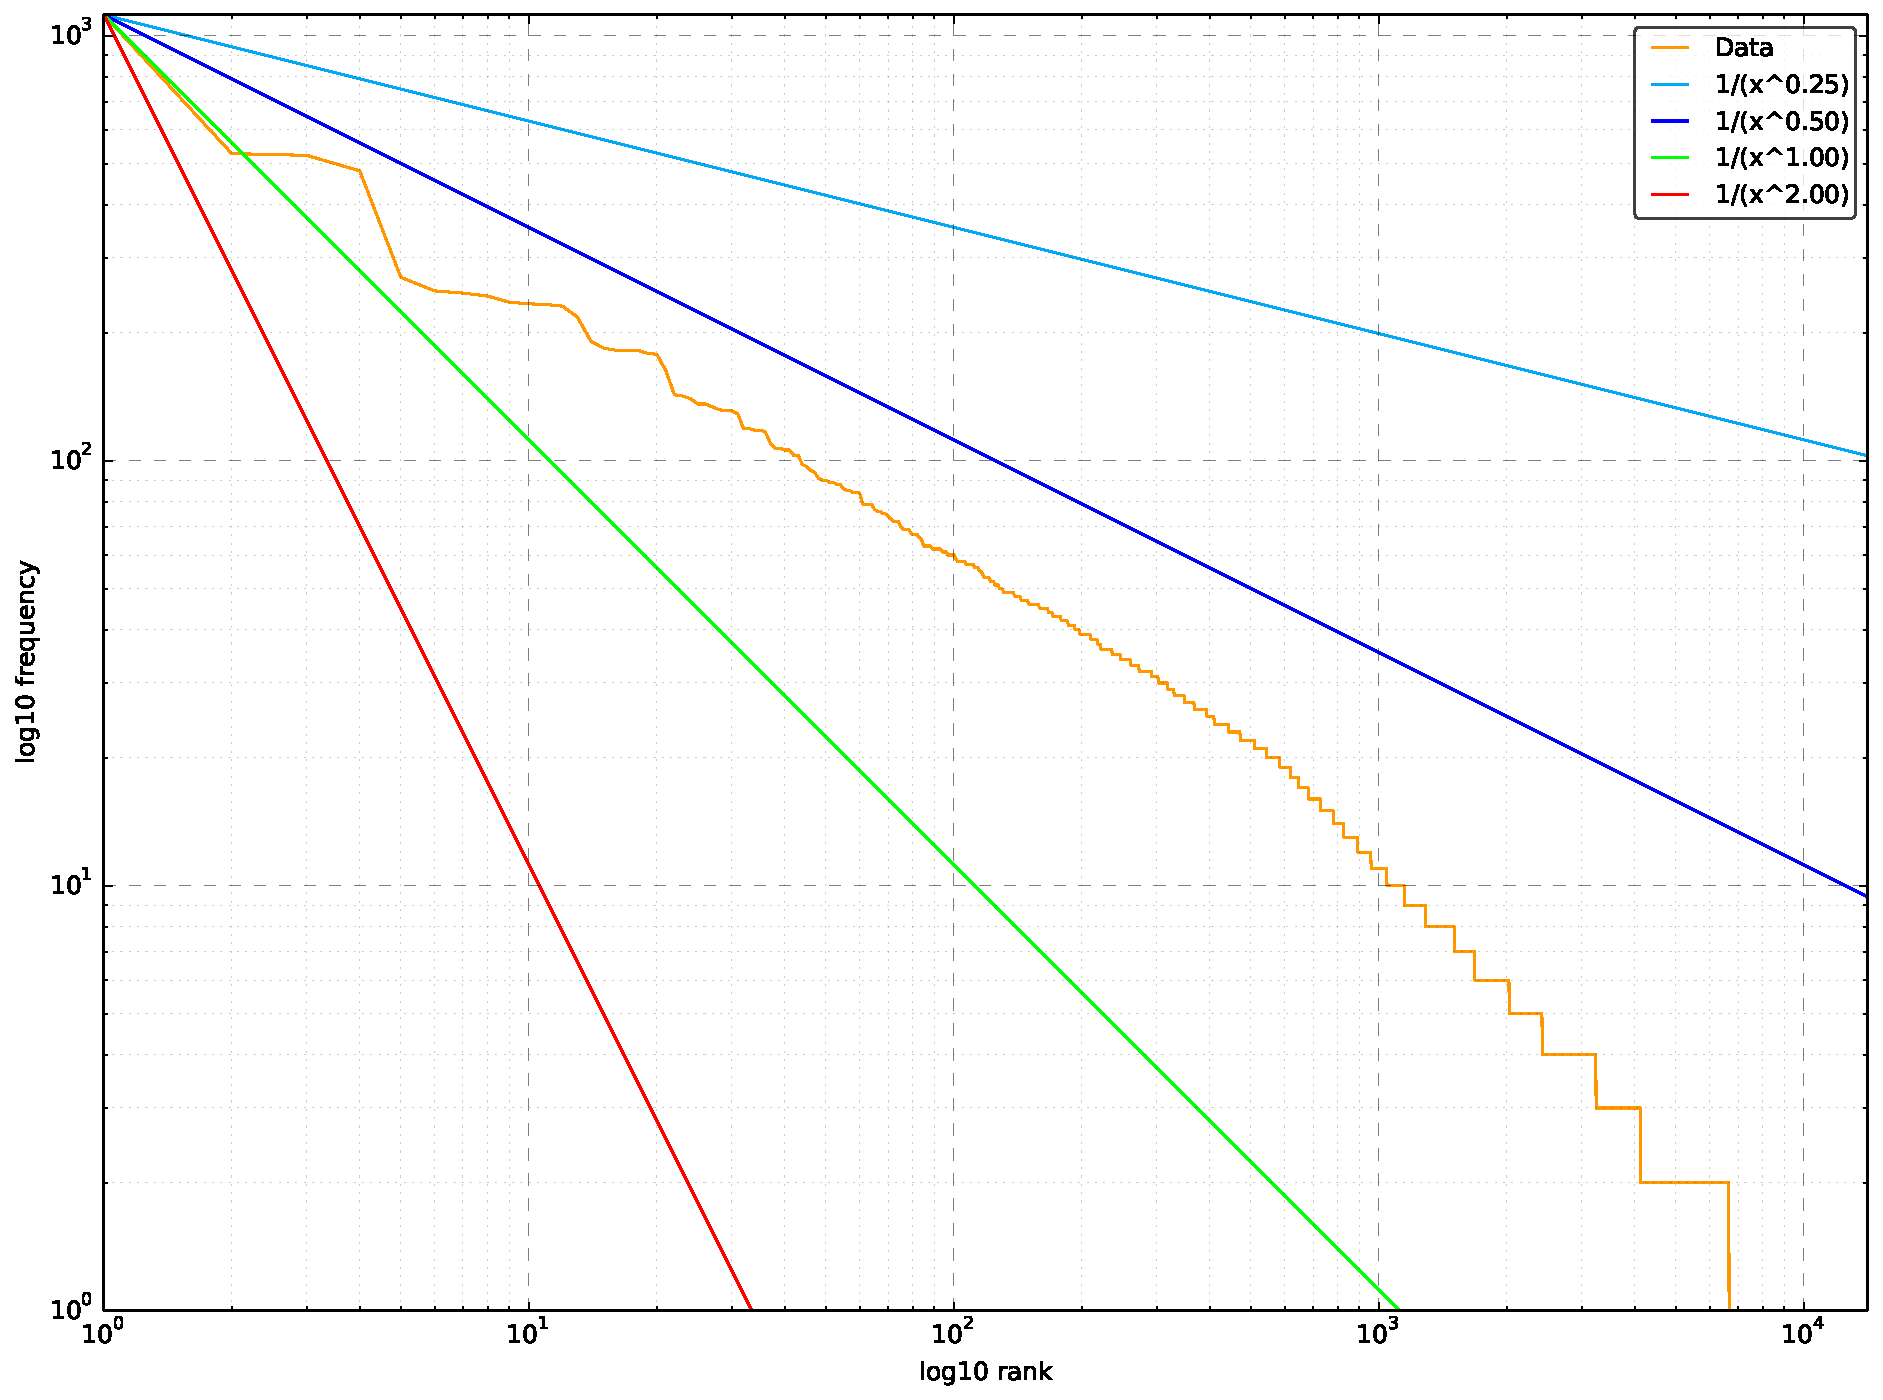
\includegraphics[width=0.9\linewidth]{figures/frequency-graphs/2-gram}
	\caption{Bigram rank-frequency graph of tokenized dataset}
	\label{fig:rank-frequency-bigram}
\end{figure}

\begin{figure}[ht]
	\centering
	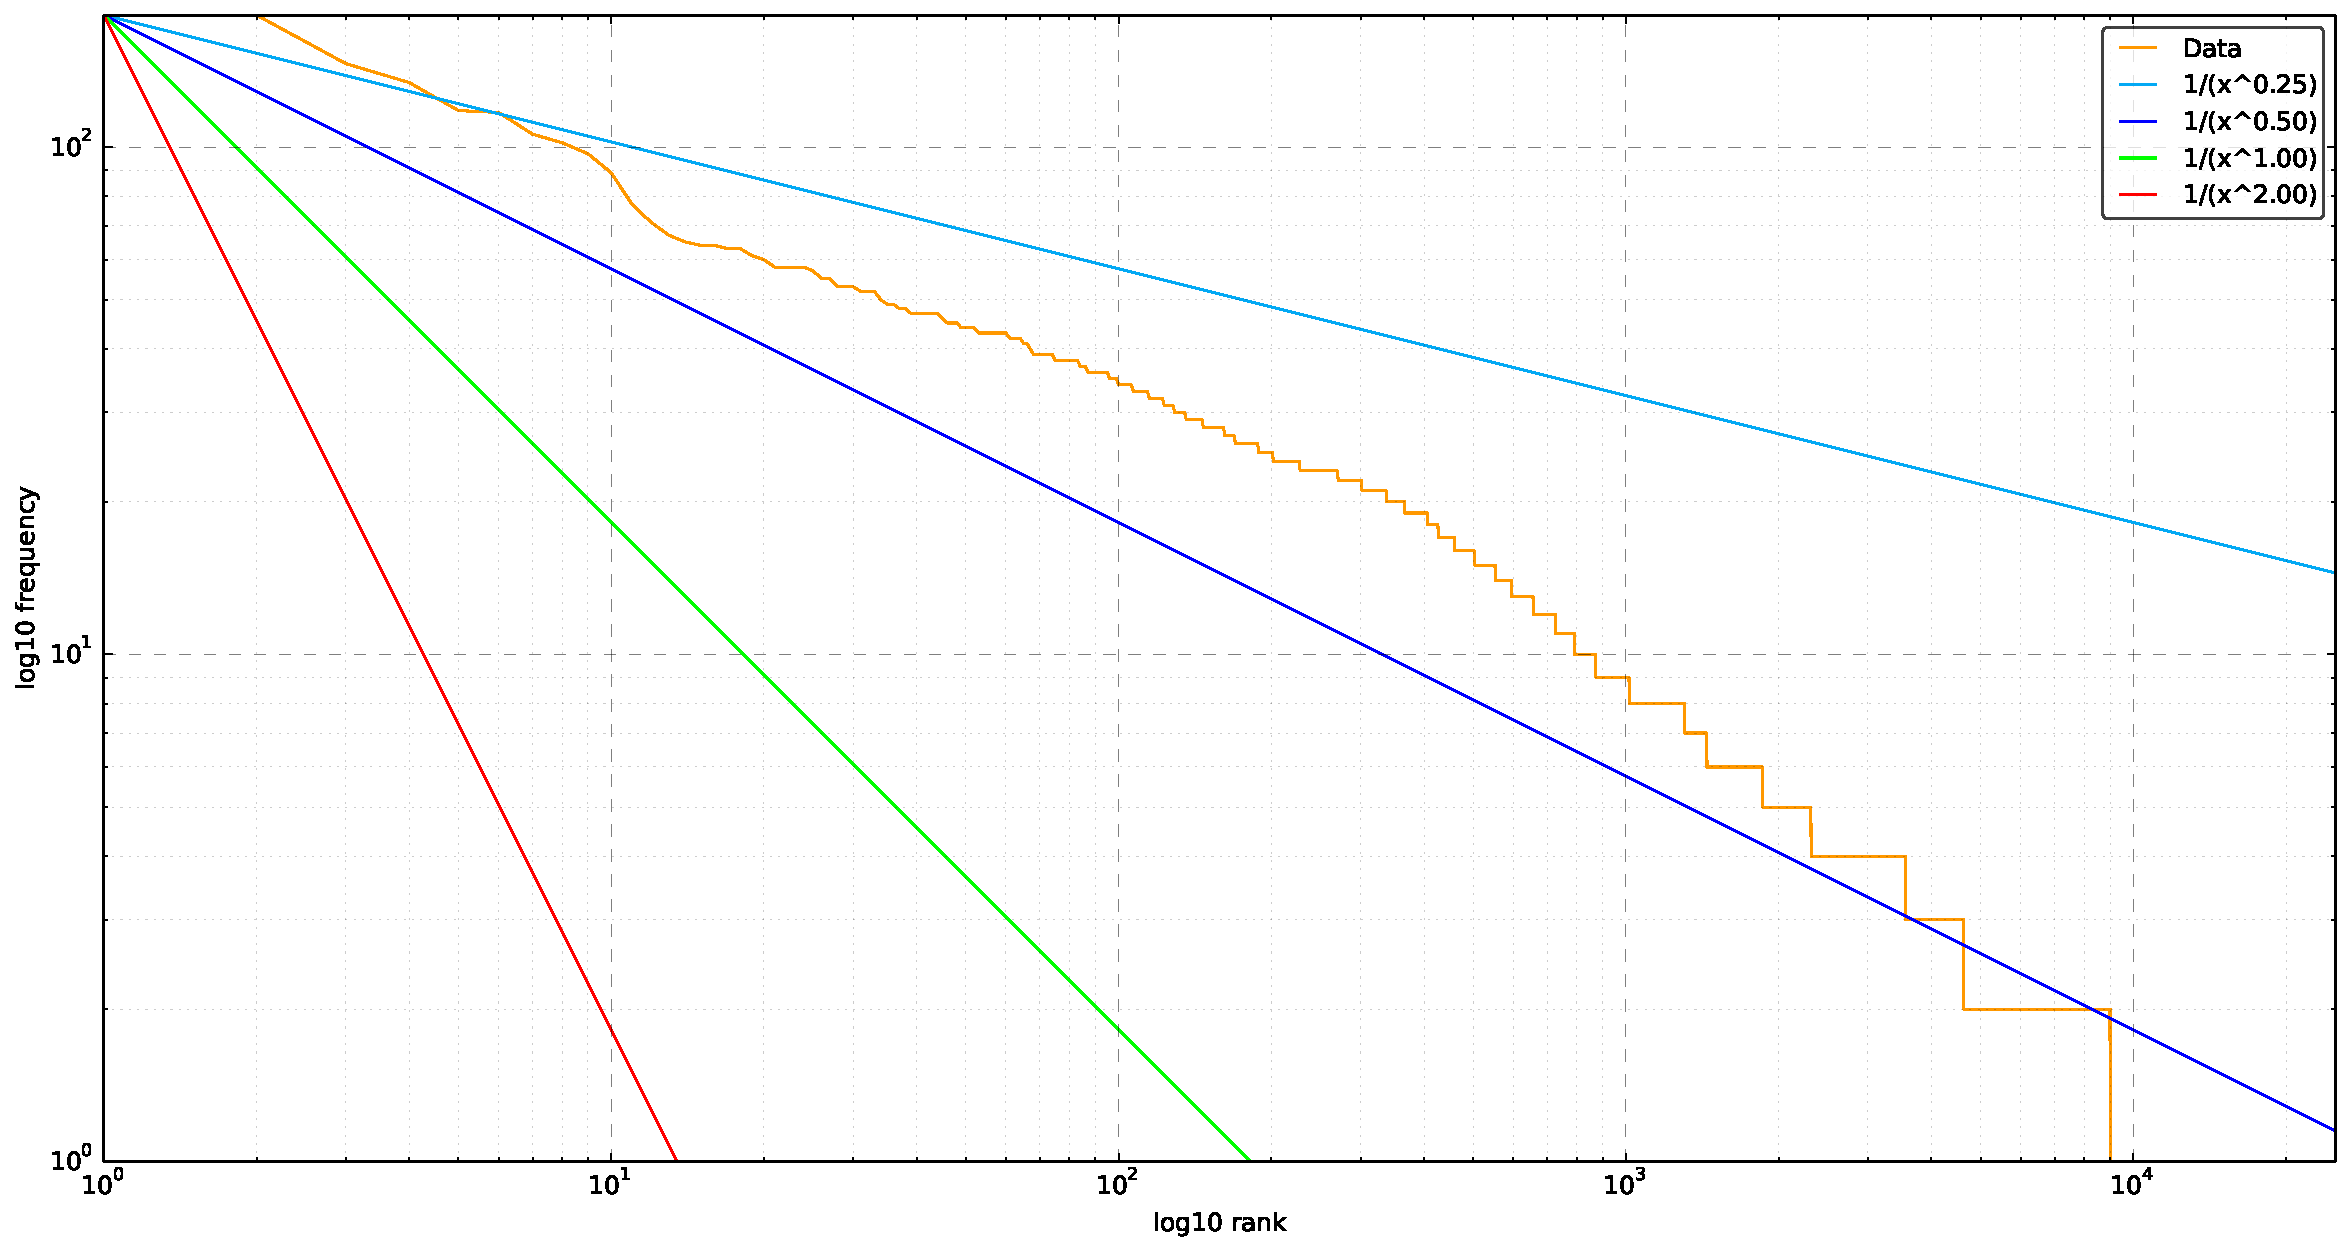
\includegraphics[width=0.9\linewidth]{figures/frequency-graphs/3-gram}
	\caption{Trigram rank-frequency graph of tokenized dataset}
	\label{fig:rank-frequency-trigram}
\end{figure}

\begin{figure}[ht]
	\centering
	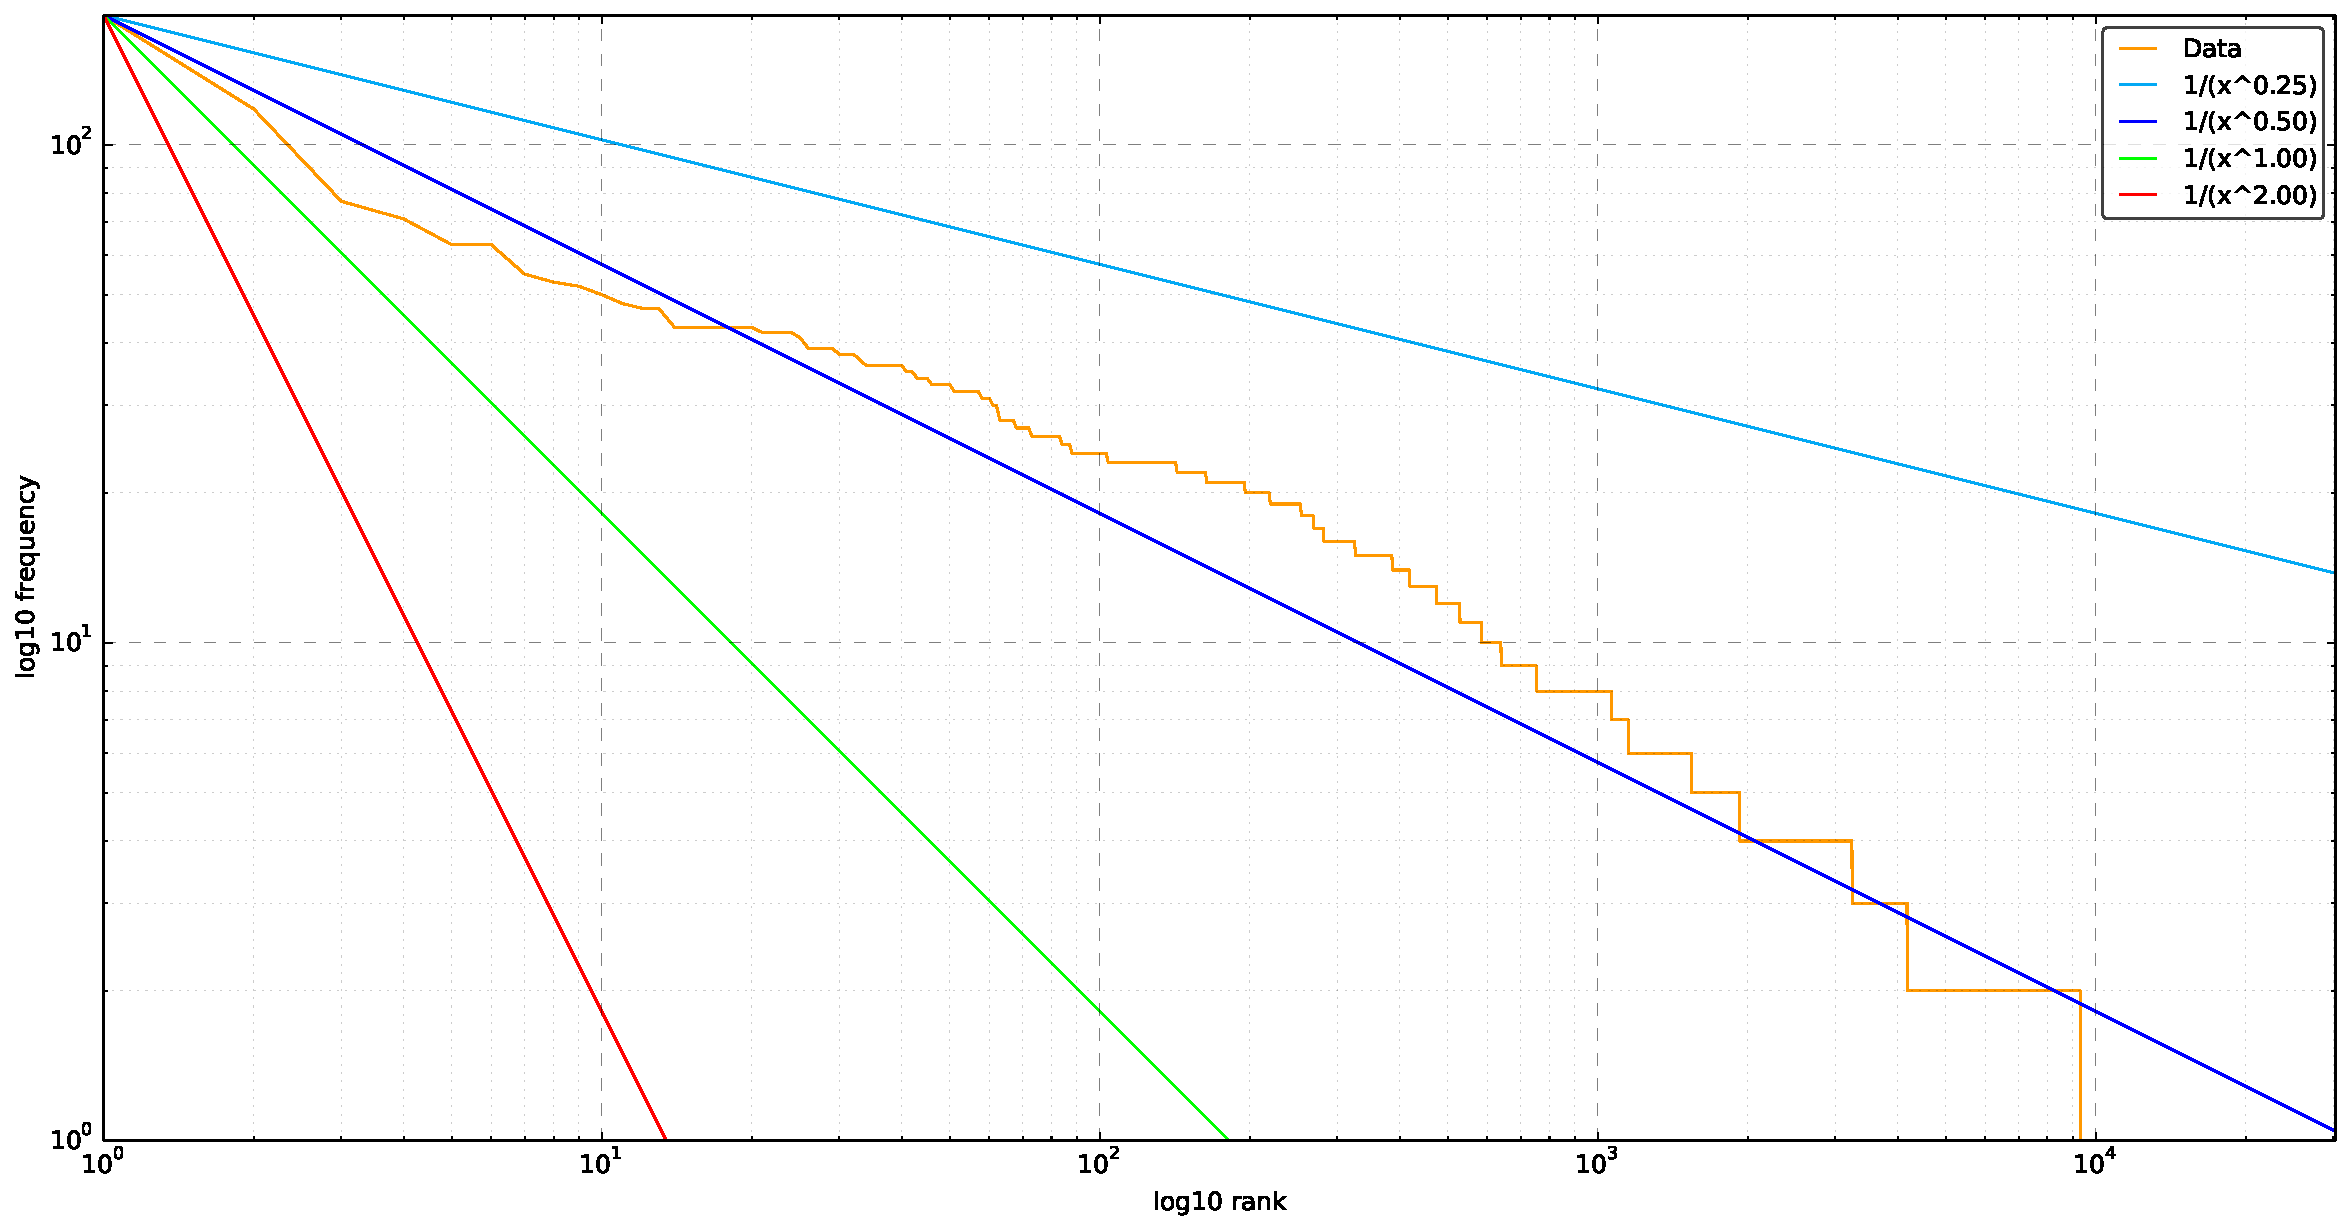
\includegraphics[width=0.9\linewidth]{figures/frequency-graphs/4-gram}
	\caption{Tetragram rank-frequency graph of tokenized dataset}
	\label{fig:rank-frequency-tetragram}
\end{figure}

\begin{figure}[ht]
	\centering
	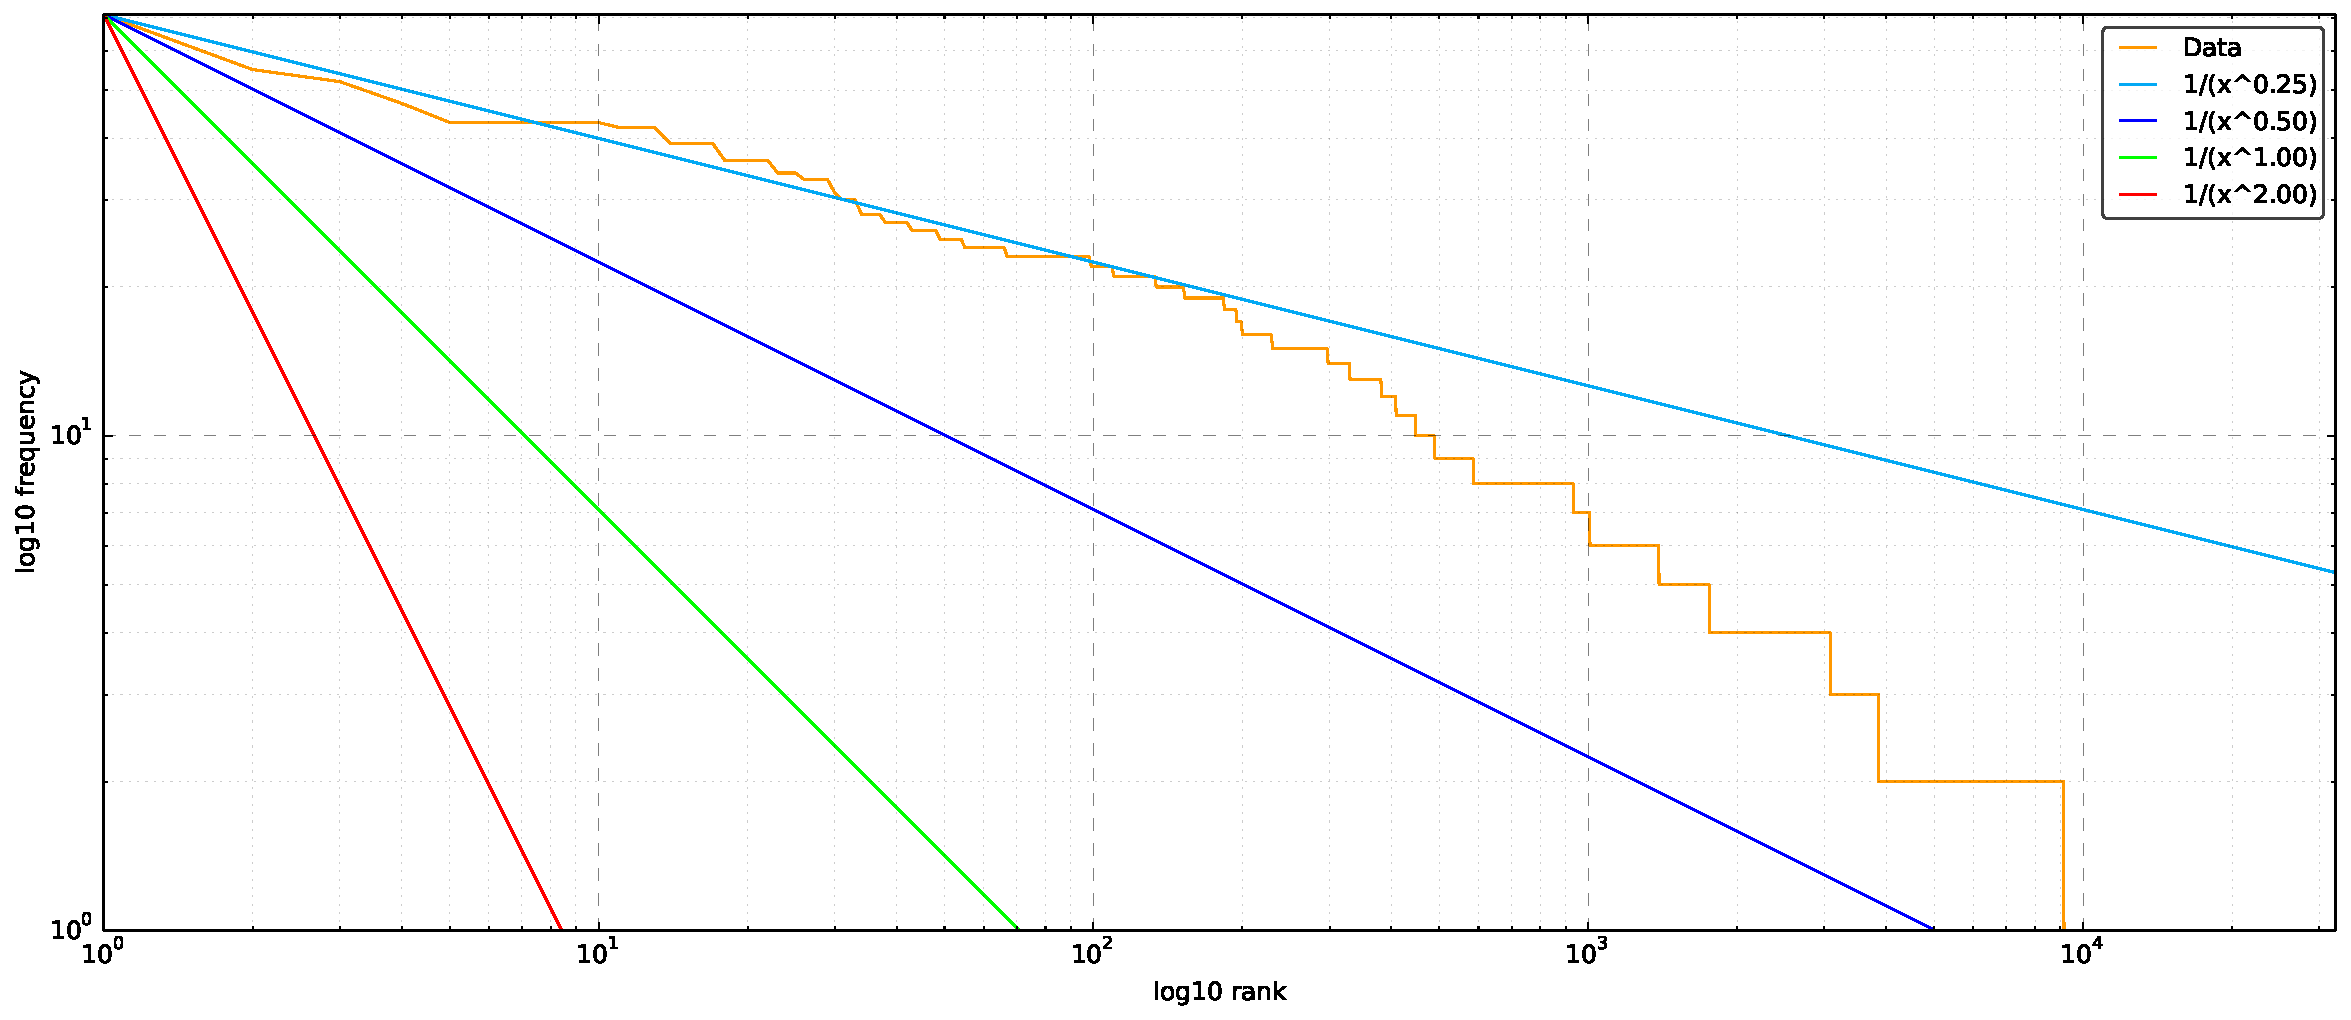
\includegraphics[width=0.9\linewidth]{figures/frequency-graphs/5-gram}
	\caption{Pentagram rank-frequency graph of tokenized dataset}
	\label{fig:rank-frequency-pentagram}
\end{figure}



\subsection{Most common and uncommon n-grams}

Analyzing the most common and uncommon words / n-grams is useful to gather a quick overview of the topics discussed in a given text corpus.

In \cref{tab:most-common-unigrams,tab:least-common-unigrams} is shown


\begin{table}[t]
	\caption{Total count of n-grams in the tokenized dataset}
	\extrarowsep = 0.47ex
	\centering
	\begin{tabu} to 0.18\textwidth { X[m,l] X[m,r] }
		\rowfont{\bfseries\itshape} N-gram & Count \\
		\hline
		Unigram		&	 2487	\\
		Bigram		&	14140	\\
		Trigram		&	25071	\\
		Tetragram	&	30346	\\
		Pentagram	& 	32409	\\
	\end{tabu}
	\label{tab:n-grams-counts}
\end{table}



\begin{table}[ht]
	\extrarowsep = 0.47ex
	\centering
	\begin{minipage}[t]{.3\linewidth}
		\caption{Most common unigrams}
		\begin{tabu} { X[2.5,m,l] X[m,r] }
			\rowfont{\bfseries\itshape} Unigram & Count \\
			\hline
			the		&	3692 \\
			.		&	3276 \\
			)		&	1745 \\
			(		&	1735 \\
			,		&	1433 \\
			</s> 	&	1357 \\
			<s>		&	1357 \\
			of		&	1235 \\
			to		&	1098 \\
			and		&	1032 \\
		\end{tabu}
		\label{tab:most-common-unigrams}
	\end{minipage}
	\hspace{2em}
	\begin{minipage}[t]{.3\linewidth}
		\caption{Least common unigrams}
		\begin{tabu} { X[2.5,m,l] X[m,r] }
			\rowfont{\bfseries\itshape} Unigram & Count \\
			\hline
			connected		&	1 \\
			disassembled	&	1 \\
			extend			&	1 \\
			fixed			&	1 \\
			heavy			&	1 \\
			motors			&	1 \\
			path			&	1 \\
			ridges			&	1 \\
			tolerance		&	1 \\
			upwards			&	1 \\
		\end{tabu}
		\label{tab:least-common-unigrams}
	\end{minipage}
\end{table}


\begin{table}[ht]
	\extrarowsep = 0.47ex
	\centering
	\begin{minipage}[t]{.4\linewidth}
		\caption{Most common bigrams}
		\begin{tabu} { X[2.5,m,l] X[m,r] }
			\rowfont{\bfseries\itshape} Bigram & Count \\
			\hline
			. </s>			&	1120 \\
			of the			&	 528 \\
			( \#			&	 523 \\
			( item			&	 481 \\
			<s> install		&	 270 \\
			main housing	&	 251 \\
			input shaft		&	 248 \\
			) .				&	 244 \\
			in the			&	 236 \\
			from the		&	 234 \\
		\end{tabu}
		\label{tab:most-common-bigrams}
	\end{minipage}
	\hspace{1em}
	\begin{minipage}[t]{.4\linewidth}
		\caption{Least common bigrams}
		\begin{tabu} { X[2.5,m,l] X[m,r] }
			\rowfont{\bfseries\itshape} Bigram & Count \\
			\hline
			engine assembly		&	1 \\
			leads to			&	1 \\
			minor adjustments	&	1 \\
			next step			&	1 \\
			open the			&	1 \\
			put lower			&	1 \\
			rotate it			&	1 \\
			sliding out			&	1 \\
			top gear			&	1 \\
			with care			&	1 \\
		\end{tabu}
		\label{tab:least-common-bigrams}
	\end{minipage}
\end{table}


\begin{table}[ht]
	\extrarowsep = 0.47ex
	\centering
	\begin{minipage}[t]{.45\linewidth}
		\caption{Most common trigrams}
		\begin{tabu} { X[2.5,m,l] X[m,r] }
			\rowfont{\bfseries\itshape} Trigram & Count \\
			\hline
			\& cone )			&	182 \\
			cup \& cone			&	182 \\
			) . </s>			&	146 \\
			pre - load			&	134 \\
			bearing pre -		&	118 \\
			bearing cone (		&	117 \\
			bearing cup (		&	106 \\
			end of the			&	102 \\
			into main housing	&	 97 \\
			main housing (		&	 89 \\
		\end{tabu}
		\label{tab:most-common-trigrams}
	\end{minipage}
	\hspace{0.5em}
	\begin{minipage}[t]{.45\linewidth}
		\caption{Least common trigrams}
		\begin{tabu} { X[2.5,m,l] X[m,r] }
			\rowfont{\bfseries\itshape} Trigram & Count \\
			\hline
			attach the piston		&	1 \\
			cutting the wires		&	1 \\
			electrical contact is	&	1 \\
			fold the conductor		&	1 \\
			install output shafts	&	1 \\
			proper function of		&	1 \\
			to the airframe			&	1 \\
			using the piston		&	1 \\
			with three screws		&	1 \\
			you push the			&	1 \\
		\end{tabu}
		\label{tab:least-common-trigrams}
	\end{minipage}
\end{table}


\begin{table}[ht]
	\extrarowsep = 0.47ex
	\centering
	\begin{minipage}[t]{.495\linewidth}
		\caption{Most common tetragrams}
		\begin{tabu} { X[4,m,l] X[m,r] }
			\rowfont{\bfseries\itshape} Tetragram & Count \\
			\hline
			cup \& cone )				&	182 \\
			bearing pre - load			&	118 \\
			bearing cone ( \#			&	 77 \\
			\& cone ) into				&	 71 \\
			bearing cup ( \#			&	 63 \\
			light coat of grease		&	 63 \\
			with light coat of			&	 55 \\
			pounds of rolling torque	&	 53 \\
			check bearing pre -			&	 52 \\
			main housing from the		&	 50 \\
		\end{tabu}
		\label{tab:most-common-tetragrams}
	\end{minipage}
	\begin{minipage}[t]{.495\linewidth}
		\caption{Least common tetragrams}
		\begin{tabu} { X[4,m,l] X[m,r] }
			\rowfont{\bfseries\itshape} Tetragram & Count \\
			\hline
			center the shaft on			&	1 \\
			connect the wire to			&	1 \\
			cutting the wires to		&	1 \\
			during the attachment of	&	1 \\
			lubricate the cam shaft		&	1 \\
			mount from the side			&	1 \\
			rod in the slot				&	1 \\
			together to make the		&	1 \\
			using the piston rod		&	1 \\
			you slide it into			&	1 \\
		\end{tabu}
		\label{tab:least-common-tetragrams}
	\end{minipage}
\end{table}


\begin{table}[ht]
	\extrarowsep = 0.47ex
	\centering
	\begin{minipage}[t]{.495\linewidth}
		\caption{Most common pentagrams}
		\begin{tabu} { X[4,m,l] X[m,r] }
			\rowfont{\bfseries\itshape} Pentagram & Count \\
			\hline
			cup \& cone ) into			&	71 \\
			with light coat of grease	&	55 \\
			check bearing pre - load	&	52 \\
			14 " to 16 "				&	47 \\
			" pounds of rolling torque	&	43 \\
			" to 16 " pounds			&	43 \\
			/ 2 to 1 hour				&	43 \\
			1 / 2 to 1					&	43 \\
			16 " pounds of rolling		&	43 \\
			to 16 " pounds of			&	43 \\
		\end{tabu}
		\label{tab:most-common-pentagrams}
	\end{minipage}
	\begin{minipage}[t]{.495\linewidth}
		\caption{Least common pentagrams}
		\begin{tabu} { X[5,m,l] X[m,r] }
			\rowfont{\bfseries\itshape} Pentagram & Count \\
			\hline
			area on shaft where seal		&	1 \\
			connect the wire to terminal	&	1 \\
			during the assembly process .	&	1 \\
			facing away from the exhaust	&	1 \\
			it is installed with two		&	1 \\
			lined up with each other		&	1 \\
			put shaft and install the		&	1 \\
			two steam inlets facing each	&	1 \\
			where it fits into the			&	1 \\
			with a screw driver ,			&	1 \\
		\end{tabu}
		\label{tab:least-common-pentagrams}
	\end{minipage}
\end{table}


\subsection{N-grams interpolation}

FF.



\subsection{N-grams models smoothing}

FF.



\subsection{Sentence generation using n-gram models}

FF.



\subsection{N-gram models perplexity}

\begin{table}[t]
	\caption{Tokenized testing dataset overview}
	\extrarowsep = 0.47ex
	\centering
	\begin{tabu} to 0.33\textwidth { X[5,m,l] X[m,r] }
		\rowfont{\bfseries\itshape} Metric & Value \\
		\hline
		Sentences							&	   439	\\
		Words								&	 20829	\\
		Out of vocabulary words ignored		&	  4848	\\
		Zero probabilities words ignored	&	  1109	\\
	\end{tabu}
	\label{tab:n-grams-models-stats}
\end{table}


\begin{table}[t]
	\caption{N-grams models perplexities}
	\extrarowsep = 0.47ex
	\centering
	\begin{tabu} to 0.29\textwidth { X[2.5,m,l] X[m,r] }
		\rowfont{\bfseries\itshape} N-gram model & Perplexity \\
		\hline
		Unigram (no smoothing)		&	243.771		\\
		Unigram (Laplace add-1)		&	245.126		\\
		Unigram (Kneser-Ney)		&	243.771		\\
		Unigram (Witten-Bell)		&	245.126		\\
		Bigram (no smoothing)		&	164.299		\\
		Bigram (Laplace add-1)		&	182.235		\\
		Bigram (Kneser-Ney)			&	 56.408		\\
		Bigram (Witten-Bell)		&	 56.717		\\
		Trigram (no smoothing)		&	133.965		\\
		Trigram (Laplace add-1)		&	233.030		\\
		Trigram (Kneser-Ney)		&	 44.559		\\
		Trigram (Witten-Bell)		&	 45.160		\\
		Tetragram (no smoothing)	&	131.832		\\
		tetragram (Laplace add-1)	&	245.794		\\
		Tetragram (Kneser-Ney)		&	 44.067		\\
		Tetragram (Witten-Bell)		&	 44.042		\\
		Pentagram (no smoothing)	&	132.059		\\
		Pentagram (Laplace add-1)	&	250.158		\\
		Pentagram (Kneser-Ney)		&	 45.725		\\
		Pentagram (Witten-Bell)		&	 44.281		\\
	\end{tabu}
	\label{tab:n-grams-models-perplexities}
\end{table}
